\documentclass[12pt]{article}

\usepackage{sbc-template}
\usepackage{graphicx,url}
\usepackage[utf8]{inputenc}
\usepackage[brazil]{babel}
     
\sloppy

\title{
  Aplicação de Algoritmos de \textit{Machine Learning} na previsão de cotação do
  \textit{Bitcoin}
}

\author{
  Rodrigo de Souza Oliveira\inst{1}, 
  Álvaro Viebrantz \inst{1}
}

\address{
  MBA em Big Data -- Fatec – Serviço Nacional de Aprendizagem Industrial (SENAI)\\
  Av. XV de Novembro, 303, Porto - CEP: 78020-300 - Cuiabá–MT
  \email{
    rddsouzaoliveira@gmail.com, 
    emaildoalvaro@gmail.com
  }
}
  
 
\begin{document} 

\maketitle

\begin{abstract}
  Resumo em inglês aqui.
\end{abstract}
     
\begin{resumo} 
Com a evolução da tecnologia e a criação de diversas ferramentas de análise de
dados, um assunto que vem se tornando muito relevante é a aplicação dessas 
técnicas avançadas de Machine Learning para entender o comportamento dos ativos 
e subsidiar o mercado financeiro de informações para tomada de decisão. Este 
trabalho teve como objetivo aplicar uma estrutura de rede neural artificial 
LSTM, com a função de analisar e entender o comportamento do bitcoin para 
projetar seu valor futuro e utilizá-lo como ferramenta para auxiliar nas 
estratégiasde investimentos. Para isso, foram coletados dados sobre a cotação 
do bitcoin, através da API de uma corretora, em uma série histórica criada desde
dezembro de 2017. Os resultados evidenciam que o modelo foi capaz de entender e 
projetar as oscilações do preço do bitcoin, porém superestimava o seu valor. 
Este trabalho abriu caminho para uma gama de possibilidades de futuros trabalhos
para melhor entender as arquiteturas de modelos disponíveis que consigam 
generalizar o comportamento do bitcoin ao longo do tempo.
\end{resumo}


\section{Introdução}

Investimento é a aplicação de algum recurso, com a expectativa de algum gannho 
futuro. A incerteza do ganho, ou um possível prejuízo, caracteria o risco do
investimeto. No contexto de aplicação financeira, pode-se caracterizar o 
investimento como a aplicação de dinheiro que não gere custos, tenha expectativa
de lucro futuro e que não exija esforços relevantes \footnote{Detalhes em Blog 
Rico. O Que é Investimento e Por Que Poupança é Ruim. Recuperado em 3 de
outubro de 2020, de \url{https://blog.rico.com.vc/o-que-e-investimento}}.

Diversos estudos, já consolidados, trazem que a diversificação do portfólio
de investimentos se demonstra como uma eficiente forma para redução dos riscos, 
conforme trazido em \cite{oda1998estudo}. A diversificação de investimentos é 
uma técnica que visa a diluição dos riscos e a maximização dos ganhos
\cite{btg:2017}.

Aliado à sua popularização nos últimos anos, o Bitcoin se tornou uma alternativa 
para os investidores comporem suas carteiras de investimentos e despertou-se a
necessidade de melhor entender seu comportamento. Porém, a oscilação e a 
incerteza do futuro do Bitcoin, gera muita insegurança, principalmente entre os 
investidores mais conservadores \cite{uol:2020}.

Como a tecnologia e as novas ferramentas de análise de dados, podem contribuir 
para transformar o bitcoin como uma alternativa de investimento, minimizando-se
os riscos das operações?

A evolução da tecnologia proporcionou o surgimento de novas ferramentas de 
análise de dados. Estas ferramentas podem contribuir para transformar o bitcoin 
como uma alternativa de investimento, pois, através do entendimento de seu 
comportamento, possibilitam a minimização dos riscos das operações com a moeda.

O Objetivo deste trabalho foi implementar e testar modelos capazes de analisar
dados históricos das cotações do Bitcoin, para identificar o comportamento do 
preço do Bitcoin e projetar as cotações futuras.

Os modelos desenvolvidos tiveram como ideia, possibilitar que o investidor tenha 
uma ferramenta técnica para auxiliar no processo de tomada de decisões sobre as 
estratégias que investimentos que serão adotadas.

Justifica-se o desenvolvimento deste trabalho, pela importância que o Bitcoin
conquistou no mercado financeiro nos últimos anos, pelo desafio na aplicação de
técnicas extremamente avançadas para análise de dados com a finalidade de prever 
o valor futuro do ativo, que é um dos grandes desafios dos cientistas de dados.

A estrutura deste trabalho está organizada da seguinte forma: 
A Metodologia (Capítulo2), onde será abordado os principais passos para 
coleta de dados, análise exploratória e o desenvolvimento do modelo, A Revisão 
de Literatura (Capítulo 3), onde serão apresentados os conceitos acerca do 
Bitcoin, Machine Learning e sobre as Redes Neurais Artificiais, A Apresentação 
da Pesquisa (Capítulo 4) e Discussão de Resultados (Capítulo 5), onde abordará 
sobre os resultados obtidos em cada etapa do desenvolvimento do modelo e o 
resultado da previsão realizada e por último, as Considerações Finais 
(Capítulo 6), onde se conclui sobre as aplicações do modelo e recomendações de 
futuros estudos.


\section{Metodologia} \label{sec:firstpage}

A finalidade dessa pesquisa tem natureza aplicada e abordagem qualitativa e 
quantitativa para realizar estudo de caráter descritivo.

Foi realizado um levantamento bibliográfico sobre os temas abordados neste 
artigo, através da coleta de informações em livros, revistas, sites e outros 
artigos.

Para a coleta e análise dos dados utilizou-se um Macbook Pro 2018 com memória 
RAM de 16GB, processador Intel i7 de 2.2Ghz, vídeo Radeon Pro 555x de 4Gb e um
Flash Storage de 251Gb, além de sistema operacional MacOS Catalina, com acesso
à internet.

Utilizou-se como linguagem de programação o R \cite{r:2020} para todas as etapas 
de análises apresentadas neste artigo e o Latex \cite{goossens93} para escrita. 
Como banco de dados, utilizou-se o Microsoft SQL Server, hospedado na nuvem 
Azure.

\subsection{Coleta dos dados}

A coleta dos dados se iniciou em dezembro de 2017, através da API REST da 
corretora de cyptomoedas Bitfinex. Estruturou-se uma rotina em linguagem R, 
dentro de uma máquina virtual no ambiente Google Cloud Plataform (GCP), 
que acessava a API e armazenava os dados em um banco de dados SQL Server, 
num período de 10 em 10 segundos.

A rotina, consultava dois grupos de informações, fornecidos pela API: 
"\textit{Ticker}" e \textit{"Orderbook"}. 
O primeiro grupo, trazia informações sobre a cotação no momento da consulta e 
trazia os seguintes campos:

\begin{itemize}
  \item Valor atual de venda
  \item Valor atual de compra
  \item Último valor negociado
  \item Menor valor negociado das últimas 24h
  \item Maior valor negociado nas últimas 24h
  \item Volume total negociado nas últimas 24h
\end{itemize}

O segundo grupo, trazia o "livro de ordens", que era a listagem de todas as 
ordens de compra e venda na corretora, vigentes no momento da consulta. 
Essa consulta retornava milhares de linhas e para reduzir o espaço de 
armazenamento, optou-se por resumir as informações antes de salvar no banco de 
dados. Os dados resumidos traziam as seguintes informações tanto das ordens de 
compra, quanto das ordens de venda:

\begin{itemize}
  \item Mínimo
  \item 1o Quartil
  \item Mediana
  \item 3o Quartil
  \item Máximo
\end{itemize}

\subsection{Análise exploratória}

Com os dados já estruturados e armazenados num banco de dados, o próximo passo
foi realizar uma análise exploratória no conjunto de dados. 

Como o tempo de resposta da API pode variar, analisou-se os intervalos entre 
cada consulta efetivamente realizada. Após essa análise, foram realizadas 
algumas tratativas nos dados para se chegar ao \textit{dataset} final.

\subsection{Modelos}

Neste trabalho foram utilizados os modelos RandomForest e 
\textit{Long-Short Term Memory} (LSTM), considerando como base de treinamento
os dados compreendidos entre novembro de 2017 até dezembro de 2019 e para 
validação os dados entre janeiro e março de 2020.

O modelo LSTM form treinado utilizando o pacote Keras \cite{chollet2015}, que 
cria uma camada para execução do ambiente Tensorflow \cite{tensorflow2015}.

\section{Revisão de Literatura}

Neste tópico serão apresentados os principais conceitos abordados no estudo,
contextualizando o Bitcoin, os tipos de aprendizados de máquina e os principais 
pontos que envolvem as redes neurais artificiais.

\subsection{Bitcoin}

O Bitcoin consiste em uma rede estruturada ponto-a-ponto, constituída por 
diversos computadores que assumem o mesmo papel de validadores das transações 
que são realizadas entre eles \cite{nakamoto2019bitcoin}.

Todas as transações que são realizadas pela rede do Bitcoin, são criptografadas,
dificultando sua rastreabilidade.

De acordo com \cite{shawn:2017}, o Bitcoin foi a primeira moeda digital a 
resolver o problema do gasto duplo, utilizando uma solução descentralizada para 
armazenamento dos registros das transações.

Outra característica da moeda é que não existe nenhum governo ou instituição que
regulamenta suas transações e seu preço. Esses fatores ajudaram a contribuir 
para a popularização do Bitcoin nos últimos anos e consequentemente a sua 
valorização, saindo de centavos de dólares em 2009 para cerca de 7 mil em 2018, 
conforme imagem abaixo.

\begin{figure}[ht]
  \centering
  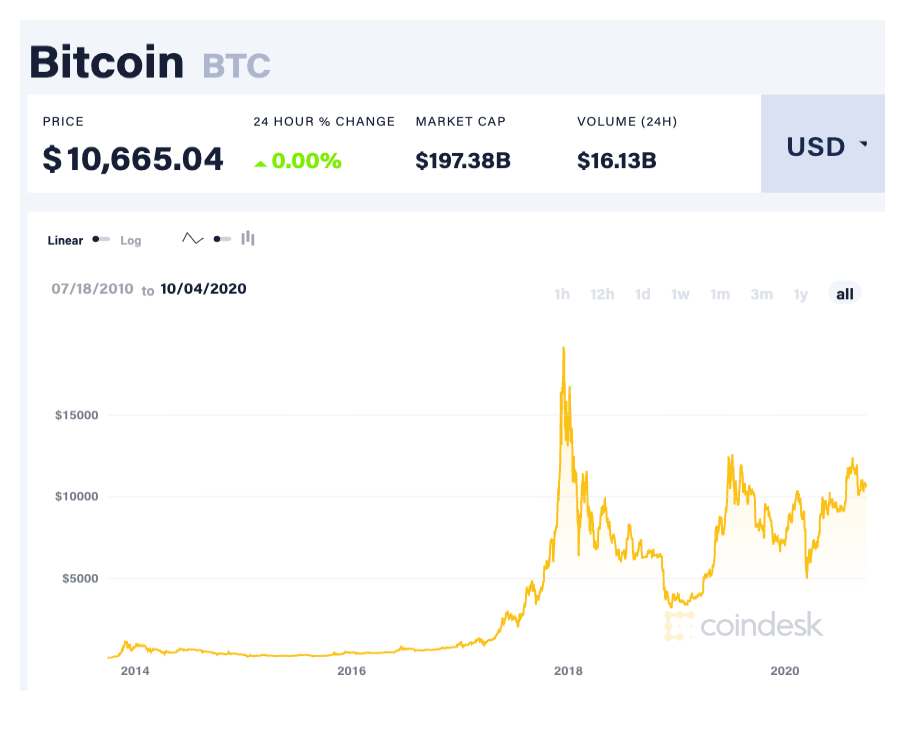
\includegraphics[scale=0.4]{img/btc-chart.png}
  \caption{Preço Histórico do Bitcoin}
  Fonte: https://www.coindesk.com/price/bitcoin
  \label{fig:btc-chart}
\end{figure}

Atualmente, estima-se mais de 375 milhões de dólares sejam comercializados em
bitcoin em apenas um dia.

\subsection{\textit{Machine Learning}}

Segundo \cite{kelleher2020fundamentals}, Machine Learning pode ser definido como 
a automação de processos que extraem padrões dos dados. Compreende um conjunto 
de técnicas computacionais que têm a característica de "aprender" com os dados.

De acordo com \cite{tanaka:2018}, existem três tipos de algoritmos de 
\textit{Machine Learning}:

\begin{itemize}
  \item \textbf{Supervisionado}: Quando se diz ao algoritmo o que é cada entrada 
  (rótulo) e ele aprende quais são as características que influenciam a entrada
  a ser o que ela é.
  \item \textbf{Não supervisionado}: Quando não se diz ao algoritmo o que é cada
  entrada, ou seja, os dados não são rotulados. O algoritmo classifica as 
  entradas conforme suas características semelhantes.
  \item \textbf{Por reforço}: Define-se um sistema de recompensas e punições aos 
  possíveis resultados para que o algoritmo possa ponderar as escolhas a serem 
  feitas.
\end{itemize}

\subsection{Redes Neurais Artificiais}

Redes Neurais Artificiais (RNAs), São modelos matemáticos, compostos por 
unidades de processamentos simples, que calculam determinadas funções 
matemáticas. Uma rede neural artificial é um modelo de computação inspirado na 
forma como a estrutura do cérebro dos mamíferos processa informação 
\cite{de2003tecnicas}.

As unidades de processamento, também chamadas de nós ou neurônios, são
dispostas em uma ou várias camadas e interligadas por conexões. 
As conexões estãoligadas a pesos, que ponderam os valores recebidos por cada 
neurônio.

O conhecimento sobre o problema em consideração está guardado dentro dos
exemplos que têm que estar obrigatoriamente disponíveis. O algoritmo de
aprendizagem generaliza esses dados e memoriza o conhecimento dentro dos
parâmetros adaptáveis da rede, os pesos \cite{rauber2005redes}.

A camada que recebe os dados é chamada de camada de entrada, a camada de saída
é responsável por traduzir o resultado da RNA e quaisquer outras são denominadas 
de camadas ocultas, ou intermediárias, vide Figura \ref{fig:nnet} abaixo. 
Em cada uma das camadas é aplicada uma função de ativação. Durante a fase de 
treinamento, a RNA "aprende" ajustando-se os pesos \cite{bishop1996neural}.

\begin{figure}[ht]
  \centering
  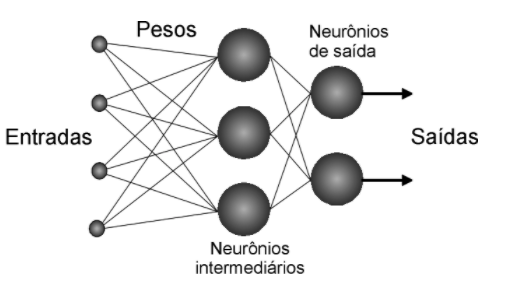
\includegraphics[scale=0.6]{img/nnet.png}
  \caption{Exemplo de uma Rede Neural Artificial de 2 camadas com 4 entradas e 2 saídas}
  Fonte: https://cerebromente.org.br/n05/tecnologia/rna.htm, \\consulta em 02 de 
  outubro de 2020
  \label{fig:nnet}
\end{figure}

\subsubsection{Redes Neurais Recorrentes e \textit{Long Short-Term Memory}}

A Rede Neural Recorrente (RNN), é uma arquitetura de rede neural especializada em
processar dados sequenciais. RNNs também são capazes de lidar com sequências de
tamanhos variados. Porém, existe uma limitação nesse tipo de rede, quando se trata
em aprender dependências após vários estágios de processamento.

Diversas variações das RNNs foram criadas com o objetivo de amenizar este
problema, sendo uma delas as células de Long Short Term Memory (LSTM). Tais
células possuem “memória”, ou seja, conseguem guardar informações por longos
períodos.

\subsection{Random Forest}

Colocar random forest ou regressão?

\section{Discussão dos resultados}

Na tabela 
\ref{summary} é possível verificar algumas estatísticas acerca do conjunto de 
dados.


% Table created by stargazer v.5.2.2 by Marek Hlavac, Harvard University. E-mail: hlavac at fas.harvard.edu
% Date and time: Sun, Oct 04, 2020 - 18:55:22
\begin{table}[!htbp] \centering 
  \caption{Sumarização dos dados} 
  \label{summary} 
\scriptsize 
\begin{tabular}{@{\extracolsep{5pt}} ccccccc} 
\\[-1.8ex]\hline 
\hline \\[-1.8ex] 
 & Min.    & 1st Qu. & Median  & Mean    & 3rd Qu. & Max.    \\ 
\hline \\[-1.8ex] 
     AIL &  3278   &  6384   &  7797   &  7917   &  9442   & 19891   \\ 
     AQ1 &  3561   &  6890   &  8217   &  8456   &  9877   & 20542   \\ 
     AMD &  3706   &  7838   &  8889   &  9357   & 11202   & 22125   \\ 
     AQ3 &  3874   &  8442   & 10762   & 11031   & 12926   & 25195   \\ 
     ASL &  4219   &  9371   & 13501   & 14550   & 19359   & 36100   \\ 
     BIL &     0   &  1783   &  4111   &  4511   &  7300   & 10475   \\ 
     BQ1 &  1001   &  4350   &  6108   &  6110   &  7863   & 13026   \\ 
     BMD &  2822   &  5448   &  6979   &  6917   &  8528   & 16156   \\ 
     BQ3 &  3067   &  5977   &  7412   &  7437   &  9097   & 18124   \\ 
     BSL &  3278   &  6384   &  7797   &  7916   &  9441   & 19890   \\ 
   BAMOUNT &    789.5   &   3785.3   &   9342.7   & 141543.1   & 129697.3   & 835193.2   \\ 
   AAMOUNT &   923.5   &  4961.4   &  7571.0   &  7961.8   & 10788.1   & 20640.8   \\ 
     Bid &  3278   &  6384   &  7797   &  7916   &  9441   & 19890   \\ 
     Ask &   3278   &   6384   &   7797   &   7918   &   9442   & 800000   \\ 
     Last &  3278   &  6384   &  7797   &  7916   &  9442   & 19891   \\ 
     Low &     0   &  6252   &  7502   &  7644   &  9183   & 18734   \\ 
     High &     0   &  6519   &  8049   &  8169   &  9725   & 19891   \\ 
    Volume &      0   &   7102   &  13983   &  23613   &  31641   & 213851   \\ 
   datetime & 2017-11-22 22 & 2018-06-25 11 & 2019-02-11 10 & 2019-01-31 06 & 2019-09-06 16 & 2020-09-29 02 \\ 
\hline \\[-1.8ex] 
\multicolumn{7}{l}{Fonte: Dados do estudo} \\ 
\end{tabular} 
\end{table} 


\section{Considerações finais}

The subsection titles must be in boldface, 12pt, flush left.

\section{Referências}

\bibliographystyle{sbc}
\bibliography{tcc-bib}

\end{document}
